
Percurso cognitivo (do inglês, \emph{Cognitive Walkthrough}), criado por
\citeonline{Wharton:1994:CWM:189200.189214} é um método de inspeção de
usabilidade utilizado para identificar problemas em sistemas interativos.
A avaliação heurística (do inglês, \emph{Heuristic Evaluation}), criado
por \citeonline{Nielsen:1990:HEU:97243.97281}, é um método de inspeção
de usabilidade utilizado para identificar problemas no
\emph{design} da interface de usuário.
O Método de Inspeção Semiótica (MIS) e o Método de Avaliação de 
Comunicabilidade (MAC), da Engenharia Semiótica, tem como
objetivo analisar a qualidade da comunicação entre
\emph{designer} e usuário através da interface de sistemas interativos
\cite{deSouza:2006:SIM:1298023.1298044}.

Neste trabalho o protótipo desenvolvido foi avaliado utilizando o 
percurso cognitivo, a avaliação heurística, MIS e MAC, para avaliar
a comunicabilidade e a usabilidade.

\subsection{Percurso cognitivo}

Porção do sistema escolhida: Acessar a lista de consultas realizadas.

Passo único: Abrir o aplicativo doutor pecúlio, a lista de consultas recentemente realizada esta 
na pagina inicial do aplicativo.

\begin{itemize}
\item O usuário tentará atingir a meta correta?
    \begin{itemize}
    \item Dada a decomposição de uma tarefa em sub-tarefas, o usuário saberá por onde começar? 
        Saberá qual é o próximo passo? \\
        Não existem sub-tarefas, a única tarefa é abrir o aplicativo.
    \item O que o usuário vai tentar fazer a cada momento?
        Navegar pela lista de consultas tocando na tela e visualizando as ultimas consultas realizadas.
    \end{itemize}
\item O usuário perceberá que a ação correta está disponível na interface?
    \begin{itemize}
        \item Onde está o elemento de interface correspondente ao próximo passo? O usuário pode vê-lo 
            ou sabe onde ele está? \\
        Só existe um paço que é abertura do aplicativo,
    \item Que ações a interface torna disponíveis? \\
       Este passo se torna desnecessário.
    \end{itemize}
\item Uma vez encontrado o elemento de interface, o usuário reconhecerá que ele produzirá o 
efeito desejado?
    \begin{itemize}
        \item O elemento de interface revela seu propósito e comportamento? \\
        Sim uma vez que a lista de consulta está disponibilizada logo no inicio do aplicativo.
    \item O usuário consegue identificar os elementos de interface? \\
      O usuário não enfrenta grandes dificuldades, pois a tarefa é simples.
    \end{itemize}
\item Após a ação correta ser executada, o usuário perceberá que progrediu em direção à solução 
da tarefa?
    \begin{itemize}
        \item Como a interface apresenta o resultado de cada ação? \\
        Nesta ação apenas aparece na tela a lista de consultas passadas. 
    \item O resultado apresentado tem correspondência com o objetivo do usuário? \\
      O protótipo é viável.
    \end{itemize}
\end{itemize}

\subsection{Avaliação heurística}

\par \noindent \textbf{Elemento da interface:} Lista de consultas já realizadas.
\par \noindent \textbf{Localização:} Tela inicial.
\par \noindent \textbf{Heurística violada:} Falta de contraste entre e fundo e cores.
\par \noindent \textbf{Gravidade:} 1 -- cosmético.
\par \noindent \textbf{Recomendação de solução:} Utilizar cores vivas.

\subsection{Método de Inspeção Semiótica (MIS)}

Os mentores deste trabalho, avaliam como é comunicação na porção aonde aparece a o item 
``Procurando...'', encontrado na tela à direita da
figura \ref{fig:TelaHistorico}, o programador quer passar pro usuário que o produto está sendo procurado 
na \emph{internet}, como objetivo da inspeção semiótica é identificar a ruptura na comunicação dos 
elementos de uma interface.

Cenário: Um usuário hipotético, alfabetizado, mas que recém comprou um 
\emph{smartphone} e não tem 
muita perícia com o equipamento, resolve tirar uma foto de um livro e nas opções de 
compartilhar escolhe o aplicativo Doutor Pecúlio, semelhante à 
figura \ref{fig:TelaHistorico} à direita. A mensagem 
do \emph{designer} quando colocou ``procurando item'' e deixou a foto em segundo plano, 
foi com o objetivo de
mostrar que o sistema estava procurando o produto que teve a foto tirada.
 O autores calculam que o tempo necessário para o recebimento
de uma resposta é de até três segundos.
Se o sistema demorar muito, ele pode achar que não conseguiu realizar esta tarefa, que o 
sistema travou, e então, sai do aplicativo e começa todo processo novamente, a ruptura na 
comunicação ocorreu quando o sistema deveria dar um indicativo de que estava trabalhando, 
ou algo do gênero.

\subsection{Método de Avaliação de Comunicabilidade (MAC)}

\par \noindent
\begin{enumerate}
\item Preparação
    \begin{itemize}
    \item Definição dos objetivos da investigação; \\
        Avaliar se o usuário é capaz de visualizar o que já havia consultados.
    \item Escolha dos participantes; \\
        A escolha é o próprio autor da avaliação, Lucas José Campos 
        Lorenzetti.
    \item Elaboração de roteiro de observação do teste; \\
        O roteiro será observando se existem dificuldades do usuário em entender que 
        naquela porção do sistema é que se localizam as suas consultas já realizadas.
    \item Executar teste-piloto; \\
        A tela utilizada foi a tela à esquerda da figura \ref{fig:TelaHistorico}.
    \end{itemize}
\item Aplicação
    \begin{itemize}
    \item Cenário -- Narrativa envolvente na qual haja um personagem com o 
        qual os participantes do teste (usuários) possam identificar:
        \begin{itemize}
        \item Atividade que este personagem deve realizar \\
            Abrir o aplicativo doutor pecúlio e visualizar suas consultas já realizadas.
        \end{itemize}
    \item Entrevista pós-teste -- Impressões gerais do participante:
        \begin{itemize}
        \item Eliminar ambiguidades para a etiquetagem posterior \\
            Aparece a etiqueta \textsc{Socorro!} Se o usuário não consegue realizar a tarefa.
        \end{itemize}
    \end{itemize}
\item Interpretação
    \begin{itemize}
    \item O avaliador deve etiquetar os vídeos da interação;
    \item Etiquetar -- Colocar ``palavras na boca do usuário'' --
        Ex.: ``Cadê?'', ``Desisto'', ``Onde estou?'', ``Vai de outro jeito!'' e etc.
    \item As etiquetas identificam tipos definidos de rupturas na comunicação; \\
        \begin{figure}[h]
            \begin{minipage}{.4\textwidth}
                \hfill
                
\includegraphics[scale=.5]{LixoSono}
                \vfill
            \end{minipage} 
            \begin{minipage}{.6\textwidth}
                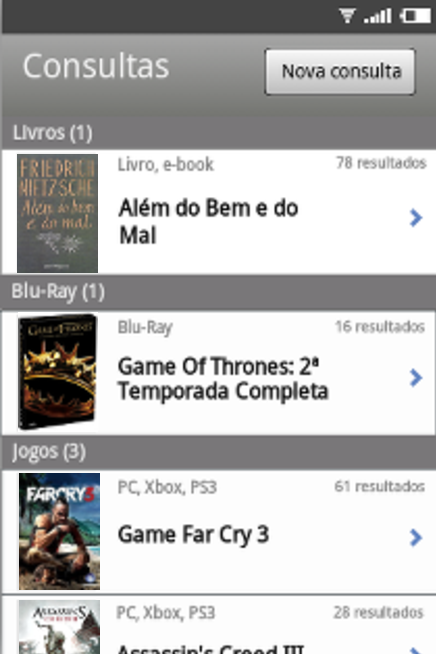
\includegraphics[scale=1]{tela/TelaHistorico}
            \end{minipage}
            \caption{Neste ponto podem surgir rupturas de comunicação.}
        \end{figure}
    \end{itemize}
\item Consolidação dos resultados
    \begin{itemize}
    \item Perguntas-guia:
    \item Qual a frequência das etiquetas por participante, por atividade (do cenário de teste), 
        por elemento da interface ou qualquer outro critério que a equipe de avaliadores 
        considerar relevante?  \\
        Podem haver no ponto inicial aonde o programa não informa
            exatamente que aquelas são as ultimas buscas.
    \item Quais padrões de ocorrência das etiquetas no contexto das atividades entre os 
        participantes?\\
        Uma vez apenas, já que foram feitos um teste piloto.
    \item Os tipos ou sequências de etiquetas podem ser associados a problemas no 
        estabelecimento das metas e submetas de comunicação? \\
        \begin{figure}[h]
            \centering
            
\includegraphics[scale=.5]{LixoMorto}
            \caption{O usuário por ventura desiste da tarefa.}
        \end{figure}
    \end{itemize}
\item Relato dos resultados
    \begin{itemize}
    \item 
        O objetivo era ver se o usuário iria conseguir saber que aquela porção era relativa a suas 
        últimas pesquisas realizadas, e a conclusão preliminar, visualizando o único caminho, após ter 
        sido aberto o \emph{software}, a etiquetagem resultou em ``socorro'' já que a função não estava 
        evidente e pode dizer ``desisto'' quando pode acreditar que não existe aquela porção do 
        sistema, a sugestão de melhoria seria então colocar um texto dizendo ``últimas consultas''
        antes de aparecerem as últimas consultas do usuário.
    \end{itemize}
\end{enumerate}

